\section{Ziel}
In diesem Versuch werden mit Hilfe von Ultraschallmessmethoden die Schallgeschwindigkeit in Acryl bestimmt und Fehlstellen in einem Acrylblock ermittelt.
Außerdem wird ein Brustmodell auf Lage und Größe von Tumoren untersucht. 



\section[Theorie]{Theorie\footnote[1]{Unter Verwendung von \cite[]{man:us1}}}

\subsection{Schallwellen}
Allgemein sind Schallwellen longitudinale Wellen, die durch Druckschwankungen
\begin{align}
    p(x,t) = p_0 + v_0 Z \cos(\omega t - kx)
    \label{eq:welle}
\end{align}
beschrieben werden können.
Dabei setzt sich die akustische Impedanz (auch Schallkennwiderstand) $Z = c \rho$ aus der Schallgeschwindigkeit im Material $c$ und der Dichte $\rho$ des Materials zusammen.
Im Gegensatz zu elektromagnetischen Wellen ist die Phasengeschwindigkeit des Schalls durch die Druck- und Dichteänderungen materialabhängig.
In Flüssigkeiten und Gasen sind Schallwellen reine longitudinale Wellen, die die Schallgeschwindigkeit
\begin{align}
    c_\text{fl} = \sqrt[]{\frac{1}{\kappa \rho}}  
    \label{eq:c-fluid}
\end{align}
haben. 
Dabei ist $\kappa$ die Kompressibilität des Fluids.
In Festkörpern sind aufgrund der Schubspannungen der Moleküle auch transversale Wellen möglich.
Für die Schallgeschwindigkeit in Festkörpern gilt
\begin{align}
    c_\text{fe} = \sqrt[]{\frac{E}{\rho}},
    \label{eq:c-fest}
\end{align}
wobei das Elastizitätsmodul $E$ und somit auch die Schallgeschwindigkeit richtungsabhängig sind.



\subsubsection{Absorption, Reflexion, Transmission}
Ein Teil der Energie geht bei der Ausbreitung einer Schallwelle durch Absorption verloren.
Für die Intensität $I_0$ gilt dabei der Zusammenhang 
\begin{align}
    I(x) = I_0 \cdot \exp(\alpha x)
    \label{eq:absorption}
\end{align}
mit dem Absorptionskoeffizienten $\alpha$.

\noindent
Beim Auftreffen einer Schallwelle auf eine Grenzfläche wird die einfallende Welle teils reflektiert und teils transmittiert.
Das Verhältnis aus reflektierter und einfallender Schallintensität wird durch den Reflexionskoeffizienten 
\begin{align}
    R = \left(\frac{Z_1 - Z_2}{Z_1 + Z_2}\right)^2
    \label{eq:reflexion}
\end{align}
beschrieben, wobei $Z_1$ und $Z_2$ je die akustischen Impedanzen der Medien sind.
Für den Transmissionskoeffizienten gilt 
\begin{align}
    T = 1 - R.
    \label{eq:transmission}
\end{align}


\subsubsection{Schallgeschwindigkeit in Luft, Wasser und Acryl}
\label{sec:schallgeschwindigkeit}
Nach \cite[]{schall-wasser-luft} hat Luft bei $\qty[]{20}{\celsius}$ eine Schallgeschwindigkeit von $c_\text{Luft} = \qty[]{344}{\meter\per\second}$
und Wasser eine Geschwindigkeit von $c_\text{Wasser} = \qty[]{1490}{\meter\per\second}$.
Außerdem hat nach \cite[]{schall-acryl} Acryl die Geschwindigkeit $c_\text{Acryl} = \qty[]{2730}{\meter\per\second}$.



\subsection{Ultraschall}

\subsubsection{Frequenzbereich}
Ultraschall befindet sich in einem Frequenzbereich von $\qty[]{20}{\kilo\hertz}$ bis $\qty[]{1}{\giga\hertz}$.
D.h. die Frequenz von Ultraschall liegt oberhalb dem für Menschen hörbaren Bereich von $\qty[]{16}{\hertz}$ bis $\qty[]{20}{\kilo\hertz}$,
und unterhalb des Hyperschalls.

\subsubsection{Wellenlänge und Periode in Acryl}
Mit Hilfe der Schallgeschwindigkeit in Acryl von $c_\text{Acryl} = \qty[]{2730}{\meter\per\second}$ (vgl. \cite[]{schall-acryl})
können bei gegebener Frequenz $\nu$ die Wellenlänge $\lambda  = c_\text{Acryl} / \nu$ und Periode $T = 1 / \nu$ ermittelt werden.
Die Werte sind in Tabelle \ref{tab:wellenlaenge-periode} zu sehen.

\begin{table}[H]
    \centering
    \caption{Wellenlänge und Periode in Acryl bei gegebener Frequenz.}
    \label{tab:wellenlaenge-periode}
    \begin{tabular}{S[table-format=1.0] S[table-format=1.4] S[table-format=1.2]}
        \toprule
        {$\nu / \unit[]{\mega\hertz}$} & {$\lambda / \unit[]{\milli\meter}$} & {$T / \unit[]{\micro\second}$} \\
        \midrule
        1 & 2.7300 & 1.00 \\
        2 & 1.3650 & 0.50 \\
        4 & 0.6825 & 0.25 \\
        \bottomrule
    \end{tabular}
\end{table}
    %lamda:  0.00273 0.001365 0.0006825
    %periode:  1e-06 5e-07 2.5e-07
    

\subsubsection{Erzeugung}
Ultraschall kann z.B. unter Anwendung des piezoelektrischen Effektes geschehen.
Hierfür wird ein piezoelektrischer Kristall in ein elektrisches Wechselfeld gebracht und zum Schwingen angeregt, 
wenn eine polare Kristallachse parallel zum äußeren Feld steht.
Beim Schwingen werden dann Ultraschallwellen emittiert.
Im Resonanzfall können hohe Schwingungsamplituden und damit hohe Schallenergiedichten erreicht werden.
Piezokristalle können auch umgekehrt durch Schallwellen zum Schwingen angeregt werden und folglich ein elektrisches Feld erzeugen.
Trotz eines relativ schwachen piezoelektrischen Effekts sind Quarze durch ihre gleichbleibenden physikalischen Eigenschaften
gut geeignete Kristalle.


\subsubsection{Anwendung}
Ultraschall wird unter anderem in der Medizin verwendet, um Informationen über den durchstrahlten Körper zu gewinnen\footnote[2]{Es 
sei angemerkt, dass Luft Ultraschall sehr gut absorbiert.
In der Medizin wird deshalb ein Kontaktmittel zwischen Sender und zu untersuchendem Material verwendet.}.
%vlt eher durchführung
Dabei werden Laufzeitmessungen verwendet, bei denen kurzzeitige Schallimpulse ausgesendet werden.
Nach der jeweiligen Laufzeit der Impulse wird auf einer definierten Strecke der Impuls von einem Empfänger gemessen.
Es wird zwischen zwei Verfahren unterschieden, die schematisch in Abbildung \ref{fig:verfahren} zu sehen sind.

\noindent
Beim Durchschallungs-Verfahren wird der Schall am anderen Ende des Materials gemessen.
Falls eine Fehlstelle vorhanden ist, kann nur eine abgeschwächte Intensität, jedoch keine Position der Stelle ermittelt werden.

\noindent
Beim Impuls-Echo-Verfahren ist der Schallsender auch der Empfänger.
D.h. der Impuls wird an einer Grenzfläche reflektiert und detektiert.
Durch die Laufzeit $t$ können so die Lagen $s$ der Fehlstellen gemäß
\begin{align}
    s = \frac{1}{2} c t
\end{align} 
bestimmt werden.

\begin{figure}[H]%
    \begin{subfigure}{0.48\textwidth}%
        \centering%
        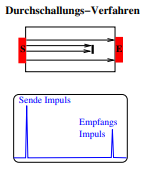
\includegraphics[height = 4cm]{abbildungen/durchschallung.png}%
        \caption{Durchschallungs-Verfahren.}%
        \label{fig:durchschallung}%
    \end{subfigure}%
    \hfill% Fills available space in the center -> space between figures
    \begin{subfigure}{0.48\textwidth}%
        \centering%
        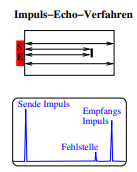
\includegraphics[height = 4cm]{abbildungen/impuls-echo.png}%
        \caption{Impuls-Echo-Verfahren.}%
        \label{fig:impuls-echo}%
    \end{subfigure}%
    \caption{Schematische Darstellungen der Ultraschallverfahren \cite{man:us1}.}%
    \label{fig:verfahren}%
\end{figure}%
\noindent

\noindent
Es gibt insgesamt drei unterschiedliche Darstellungsarten für die Laufzeitdiagramme (in der Medizin):

\noindent
Beim eindimensionalen A-Scan (A = Amplitude) wird die Echoamplituden als Funktion der Laufzeit dargestellt. 
Er wird zur Abtastung von Strukturen verwendet.

\noindent
Der B-Scan (B = Brightness) erzeugt ein zweidimensionales Bild, indem beim Bewegen der Sonde Helligkeitsabstufungen dargestellt werden.

\noindent
Beim TM-Scan (TM = Time Motion) wird eine zeitliche Bildfolge durch eine schnelle Abtastung aufgenommen.
Dadurch kann beispielsweise eine Organbewegung sichtbar gemacht werden.

